\documentclass[manuscript,anonymous,review]{acmart}
\usepackage{amsmath}

\AtBeginDocument{%
  \providecommand\BibTeX{{\normalfont B\kern-0.5em{\scshape i\kern-0.25em b}\kern-0.25em T\kern-0.1667em\lower0.7ex\hbox{E}\kern-0.125emX}}}

\title{Supplementary Material: Data Quality for Derived Preference Graphs:
  Construction Sensitivity and Repair Outcomes in Multi-Ranker Retrieval}

\author{Anonymous Author(s)}
\affiliation{%
  \institution{Institution redacted for review}
  \country{}
}

\begin{document}

\maketitle

\noindent This document is supplementary material for the main manuscript
``Data Quality for Derived Preference Graphs: Construction Sensitivity and
Repair Outcomes in Multi-Ranker Retrieval.'' It is not self-contained: every
section below expands a claim summarized in the compressed main paper, and no
result here is presented as evidence independent of the main paper's claims.
Every table and figure in this document was computed by the same released,
versioned pipeline as the main-text results (see the main paper's Data
Availability and Reproducibility section); nothing here is a new experiment.
Sections A--H group the detail moved out of the main paper during the final
page-limit compression.

% =============================================================================
\section{A. Extended Protocol Definitions}
\label{sec:supp-protocols}

Referenced from the main text's ``Threshold Protocols'' subsection,
which names four headline protocols
(\texttt{raw\_fixed}, \texttt{minmax\_raw\_matched}, \texttt{minmax\_quantile},
\texttt{rank\_percentile}) and states that, together with the
$q\in\{0.3,0.5,0.7\}$ sensitivity grid, these correspond to eight registered
protocol configurations. The joint multiplicity families additionally draw
on four further registered configurations, defined here, bringing the total
to the twelve referenced throughout the paper:

\begin{itemize}
  \item \texttt{ablation\_minmax\_fixed} -- \texttt{raw\_fixed}'s fixed
    numeric thresholds ($0.05$/$0.1$), but with min--max calibration applied
    to scores before thresholding instead of raw native scores.
  \item \texttt{ablation\_unit\_vote\_retention} -- the same fixed numeric
    thresholds, but with unit-weight votes (each retained vote contributes
    weight $1$) instead of margin-weighted votes.
  \item \texttt{robustness\_zscore\_retention} -- constructed exactly like
    \texttt{minmax\_raw\_matched} (retention-matched to \texttt{raw\_fixed}),
    but substituting per-query, per-ranker $z$-score standardization for
    min--max normalization.
  \item \texttt{robustness\_rank\_percentile\_retention} -- constructed
    exactly like \texttt{minmax\_raw\_matched}, but substituting the
    percentile transform for min--max normalization. Not to be confused
    with the independently-thresholded \texttt{rank\_percentile} protocol,
    which uses the same percentile transform but a pre-registered quantile
    threshold rather than retention-matching.
\end{itemize}

These four are reported only inside the main paper's joint multiplicity
families (``Multiplicity and Influence Robustness'' subsection) as an even
more conservative robustness check; none is a headline protocol, and none
changes the primary-protocol decision.

Referenced from the main text's ``Normalization Changes Graph Construction''
subsection. The main paper's structural-results table already reports every
value plotted below (cyclic-query percentage by dataset and regime, before
and after mutual-pair deletion); the two figures here give the same values
as grouped bar charts for visual comparison across datasets and against the
raw-margin ablation.

Referenced from the main text's ``Ranker Dependence, Mutual-Pair
Attribution, and Why \texttt{ms2} Is Acyclic'' subsection, which states in
prose that the custom TF-IDF implementation was validated against
scikit-learn's \texttt{TfidfVectorizer} and matches closely.

\textbf{TF-IDF implementation validation.} We validated our TF-IDF
implementation (described in the main paper's ``Upstream Rankers and
Candidate Pooling'' subsection) against
scikit-learn's \texttt{TfidfVectorizer}, configured to match its tokenizer,
sublinear term frequency, smoothed IDF, and $\ell_2$-normalized cosine
scoring, on a deterministic five-query sample per dataset scored against
the full document corpus. Top-$50$ ($35$ for HotpotQA) overlap is exact
(Jaccard $=1.0$) on every sampled query, score Pearson correlation on
jointly-ranked documents exceeds $0.9999$, and directional pairwise
agreement is $1.0$ on every sampled query. This does not replace the
stored canonical TF-IDF scores used throughout the paper; it confirms the
implementation used to produce them is internally correct.
Figures~\ref{fig:supp-cyclicity-scc} and
\ref{fig:supp-raw-calibrated-structure} visualize the structural cyclicity
values summarized in the main paper.

\begin{figure}[h]
  \centering
  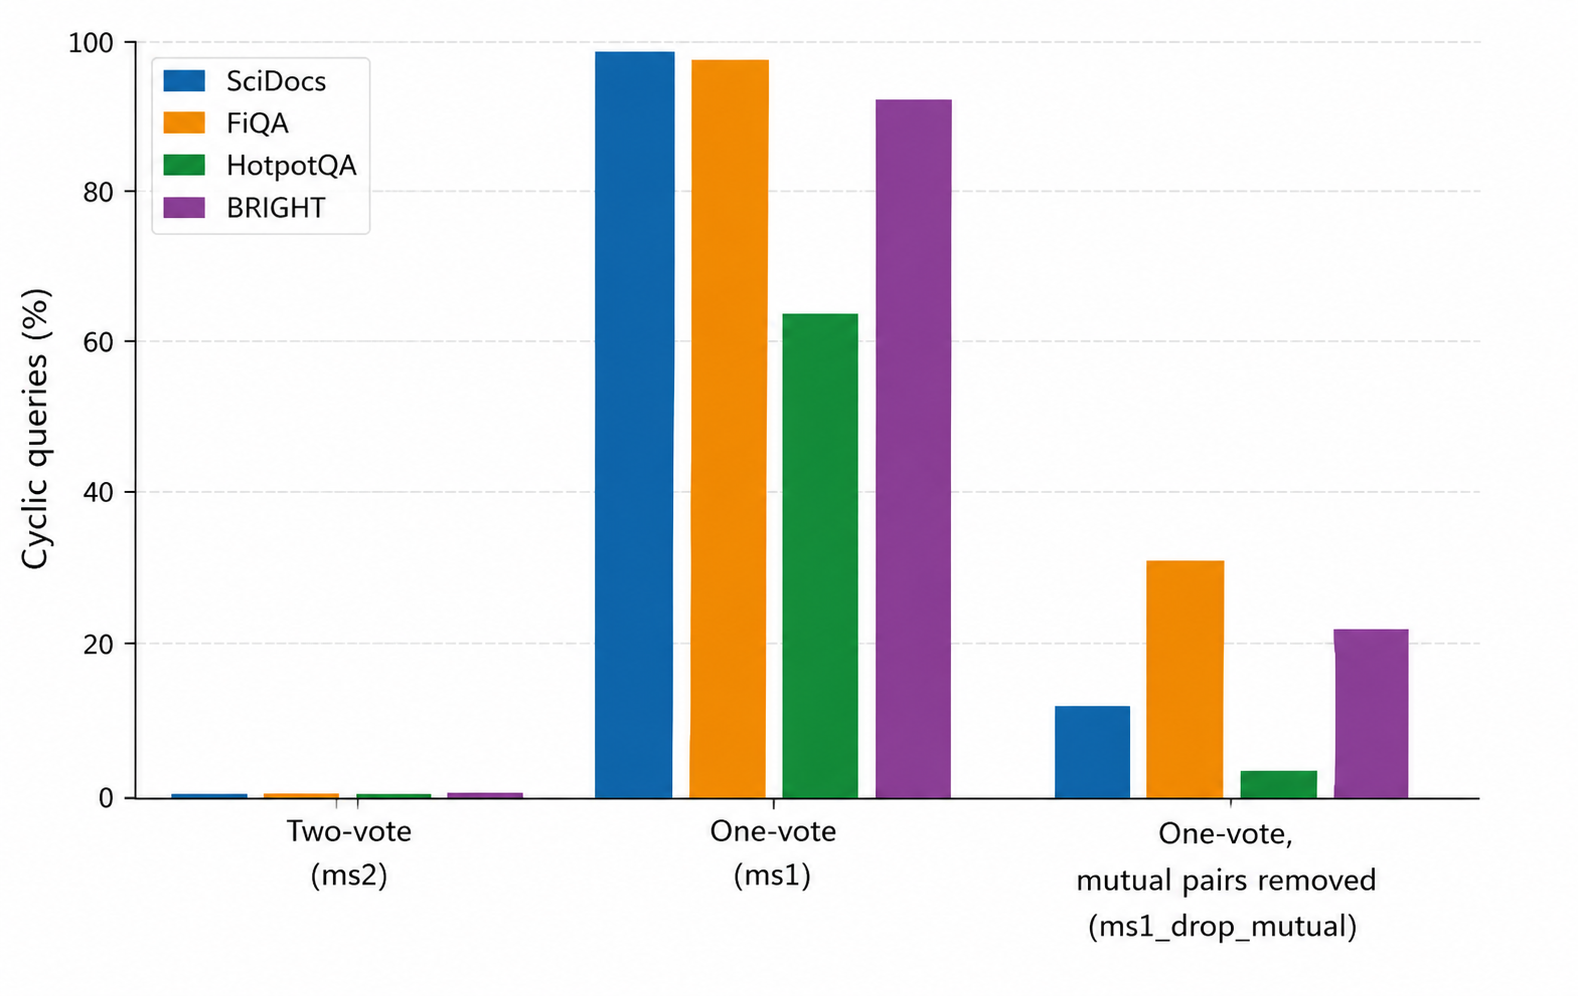
\includegraphics[width=0.8\linewidth]{figure3.png}
  \caption{Cyclic-query percentage under the primary normalized protocol,
    grouped by vote regime with one bar per dataset. \texttt{ms2} is exactly
    $0\%$ on every dataset; \texttt{ms1} is $64$--$99\%$; deleting direct
    mutual pairs (\texttt{ms1\_drop\_mutual}) brings every dataset back down
    to $2$--$31\%$, since \texttt{ms1}'s high cyclicity is concentrated almost
    entirely in direct mutual contradictions rather than longer cycles (the
    main paper's mutual-pair-deletion figure isolates that residual). Values
    before mutual-pair deletion; post-deletion values are also in the main
    paper's structural-results table.}
  \Description{A grouped bar chart of cyclic-query percentage by vote regime
    (ms2, ms1, ms1-drop-mutual) with one bar per dataset (SciDocs, FiQA,
    HotpotQA, BRIGHT) under the primary normalized protocol. ms2 is zero
    for every dataset; ms1 ranges from about 64 to 99 percent; ms1-drop-mutual
    drops back to about 2 to 31 percent.}
  \label{fig:supp-cyclicity-scc}
\end{figure}

\begin{figure}[h]
  \centering
  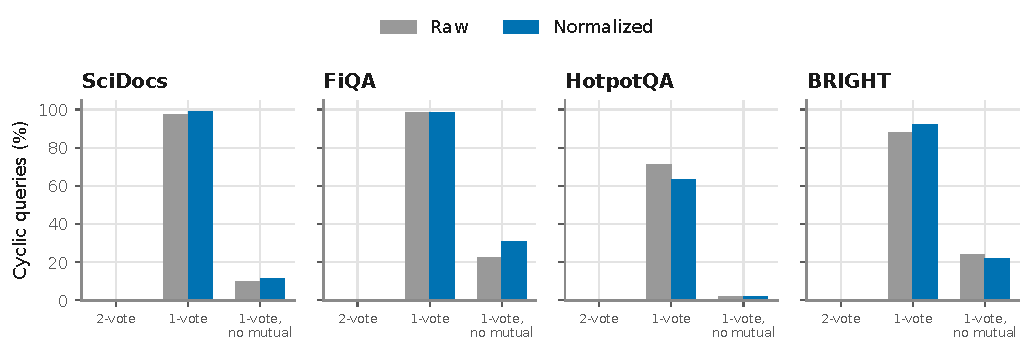
\includegraphics[width=\linewidth]{figures_v2/fig4_raw_vs_calibrated_structure.pdf}
  \caption{Cyclic-query percentage by vote regime, raw-margin ablation (gray)
    versus primary normalized protocol (blue), one panel per dataset.
    Unlike the BM25 weight share in the main paper's scale-dominance figure,
    overall
    cyclic-query rate changes only modestly between raw and normalized
    construction within each regime; this does not mean normalization leaves
    the graph unchanged, since the removed-edge overlap between raw and
    normalized repair is only $0.055$--$0.328$, so normalization changes
    \emph{which} edges are cyclic and removed far more than it changes the
    headline cyclic-query rate shown here.}
  \Description{Four grouped bar charts, one per dataset, each comparing
    cyclic-query percentage across the ms2, ms1, and ms1-drop-mutual regimes
    for the raw-margin ablation (gray) versus the primary normalized
    protocol (blue). The two protocols track each other closely within every
    regime and dataset.}
  \label{fig:supp-raw-calibrated-structure}
\end{figure}

% =============================================================================
\section{B. Full Statistical Robustness}
\label{sec:supp-statistics}

Referenced from the main text's ``Multiplicity and Influence Robustness''
subsection, which states the exact per-step influence-removal values for
both panels below in prose (HotpotQA: $+0.0123 \to +0.0053 \to +0.0009 \to
0 \to 0$ as the top 1-4 influential queries are removed; SciDocs (at
$k=0,1,2,3,4$): $+0.0085 \to +0.0055 \to +0.0036 \to +0.0048 \to +0.0041$).

Referenced from the main text's ``Alpha Sensitivity and Balance
Degeneracy'' subsection, which states in prose which datasets/$\alpha$
combinations remain positive, negative, or sign-flipping across the sweep.
Table~\ref{tab:supp-alpha-sensitivity} gives the full alpha grid, and
Figure~\ref{fig:supp-influence-robustness} shows the corresponding
query-influence sensitivity traces cited in the main text.

\begin{table}[h]
  \caption{Copeland-hybrid alpha sensitivity under the primary normalized
    protocol, \texttt{ms1} only. Entries are repaired-minus-unrepaired mean
    nDCG@$k$; this is a small sensitivity sweep, not a tuned hyperparameter
    search.}
  \label{tab:supp-alpha-sensitivity}
  \begin{tabular}{lrrrr}
    \toprule
    Dataset & $\alpha=0.1$ & $\alpha=0.3$ & $\alpha=0.5$ & $\alpha=1.0$ \\
    \midrule
    SciDocs  & $-0.0022$ & $+0.0085$ & $+0.0097$ & $+0.0083$ \\
    FiQA     & $+0.0006$ & $-0.0046$ & $+0.0010$ & $+0.0038$ \\
    HotpotQA & $-0.0008$ & $+0.0123$ & $+0.0120$ & $+0.0101$ \\
    BRIGHT   & $-0.0013$ & $+0.0006$ & $-0.0074$ & $-0.0071$ \\
    \bottomrule
  \end{tabular}
\end{table}

\begin{figure}[h]
  \centering
  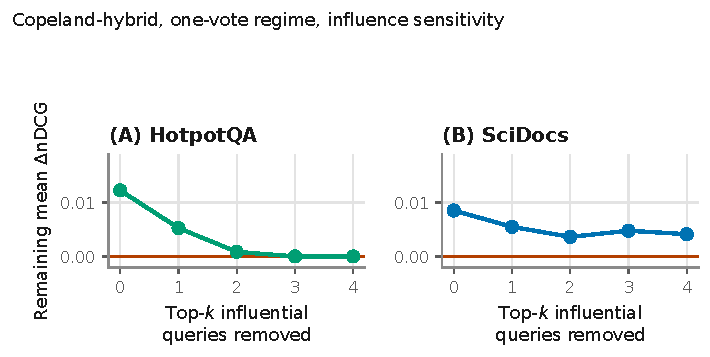
\includegraphics[width=0.85\linewidth]{figures_v2/fig8_influence.pdf}
  \caption{Remaining mean $\Delta$nDCG for the normalized \texttt{ms1}
    Copeland-hybrid cell as the top-$k$ most influential queries are removed
    ($k=0,\dots,4$), exact per-query recomputations, not interpolated.
    HotpotQA (A) is the more concentrated case: the mean falls from
    $+0.0123$ to exactly $0$ after removing the top 3 queries. SciDocs (B) is
    less concentrated and stays positive through $k=4$ ($+0.0085$ at $k=0$,
    never dropping below $+0.0036$).}
  \Description{Two line-and-marker panels. Panel A, HotpotQA, shows the
    remaining mean delta nDCG dropping from 0.0123 at k equals 0 to exactly 0
    by k equals 3 influential queries removed. Panel B, SciDocs, shows the
    remaining mean delta nDCG staying positive from 0.0085 at k equals 0 down
    to about 0.004 at k equals 4, never reaching zero.}
  \label{fig:supp-influence-robustness}
\end{figure}

% =============================================================================
\section{C. Exact Repair Analyses}
\label{sec:supp-exact}

Referenced from the main text's ``Structural Repair Activity'' subsection,
which states the same finding in prose: \texttt{ms2} removes zero weight on
every dataset by construction, \texttt{ms1} removes $0.029$--$0.080$ of
total graph weight, and \texttt{ms1\_drop\_mutual} removes only a small
residual ($\le 0.004$). Figure~\ref{fig:supp-bew-pic} gives the full
per-dataset decomposition used by that summary.

\begin{figure}[h]
  \centering
  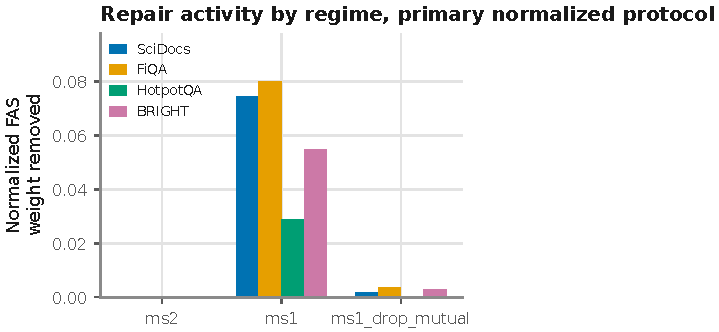
\includegraphics[width=0.8\linewidth]{figures_v2/fig6_normalized_fas_removed.pdf}
  \caption{Mean normalized FAS weight removed (removed weight divided by
    total graph weight) by vote regime, one bar per dataset, under the
    primary normalized protocol. \texttt{ms2} removes exactly $0$ on every
    dataset by construction (it is always acyclic); \texttt{ms1} removes
    $0.029$--$0.080$ of total graph weight; \texttt{ms1\_drop\_mutual} removes
    only a small residual ($\le 0.004$). This is an intrinsic graph diagnostic
    computed before any retrieval evaluation, not a measure of retrieval
    benefit.}
  \Description{A grouped bar chart of mean normalized feedback-arc-set weight
    removed by vote regime (ms2, ms1, ms1-drop-mutual), one bar per dataset,
    under the primary normalized protocol. ms2 is zero for every dataset;
    ms1 ranges from about 0.03 to 0.08; ms1-drop-mutual is a small residual
    under 0.005 for every dataset.}
  \label{fig:supp-bew-pic}
\end{figure}

% =============================================================================
\section{D. Candidate-Pool and Cutoff Robustness}
\label{sec:supp-pool}

Referenced from the main text's ``The baseline comparison is not an
artifact of the RRF-centered candidate pool'' paragraph, which states the
headline result in prose: under the canonical pool, 0 of 8 pre-specified
Holm-corrected cells are significant, and the one nominally significant
cell across all five pools tested occurs under the neutral round-robin
pool, not the canonical one -- the opposite of a home-field-advantage
pattern.

Referenced from the main text's ``Conditional Analysis and Failure
Decomposition'' subsection, which restates every value below in prose while
walking through the nested-subset funnel for the HotpotQA \texttt{ms1}
Copeland-graph cell at $(P,k)=(35,10)$. Tables~\ref{tab:supp-conditional-hotpotqa}
and \ref{tab:supp-pool-fairness} hold the moved conditional and pool-fairness
detail.

\begin{table}[h]
  \caption{Conditional decomposition of the HotpotQA \texttt{ms1}
    Copeland-graph cell at $(P,k)=(35,10)$ ($52$ queries total). Sample size
    and mean
    $\Delta$nDCG for each nested subset.}
  \label{tab:supp-conditional-hotpotqa}
  \scriptsize
  \begin{tabular}{lrr}
    \toprule
    Subset & $n$ & Mean $\Delta$nDCG \\
    \midrule
    All queries                                   & 52 & $+0.0165$ \\
    Has a cycle / repair active                   & 44 & $+0.0195$ \\
    Repaired ranking differs from unrepaired      & 43 & $+0.0200$ \\
    Top-$k$ document \emph{set} changes           & 19 & $+0.0219$ \\
    Qrels-labeled document ordering changes       & 8  & $+0.0854$ \\
    \bottomrule
  \end{tabular}
\end{table}

\begin{table}[h]
  \caption{Targeted paired comparison of \{RRF, CombSUM\} vs.\ the fixed
    repaired Copeland hybrid (\texttt{hybrid\_repaired\_copeland\_a0p3\_minmax}),
    \texttt{ms1} regime, mean nDCG delta (baseline minus graph method). The
    primary canonical-pool family (8 cells) is Holm-corrected jointly and is
    the only family used for an inferential claim; the neutral-pool column is
    reported for robustness context only. Full five-pool results are in the
    released artifact.}
  \label{tab:supp-pool-fairness}
  \scriptsize
  \begin{tabular}{llrrrr}
    \toprule
    Dataset & Baseline & \multicolumn{2}{c}{Canonical (RRF) pool} & \multicolumn{2}{c}{Neutral pool} \\
     & & $\Delta$ nDCG & Holm $p$ & $\Delta$ nDCG & Holm $p$ \\
    \midrule
    SciDocs  & RRF     & $-0.0066$ & $0.625$ & $-0.0058$ & $0.863$ \\
    SciDocs  & CombSUM & $-0.0099$ & $0.625$ & $-0.0051$ & $1.000$ \\
    FiQA     & RRF     & $+0.0141$ & $0.058$ & $+0.0082$ & $0.629$ \\
    FiQA     & CombSUM & $+0.0135$ & $0.342$ & $+0.0140$ & $\mathbf{0.013}$ \\
    HotpotQA & RRF     & $-0.0197$ & $0.625$ & $-0.0103$ & $1.000$ \\
    HotpotQA & CombSUM & $+0.0045$ & $0.625$ & $+0.0127$ & $1.000$ \\
    BRIGHT   & RRF     & $+0.0137$ & $0.342$ & $+0.0043$ & $1.000$ \\
    BRIGHT   & CombSUM & $+0.0250$ & $0.198$ & $+0.0123$ & $1.000$ \\
    \bottomrule
  \end{tabular}
\end{table}

% =============================================================================
\section{E. Ranker Dependence and Coverage}
\label{sec:supp-ranker-dep}

Referenced from the main text's ``Structural Repair Activity'' subsection,
which states in prose that, under the principled judged-pair rule, SciDocs
and HotpotQA provide usable qrels-pair diagnostics while FiQA and BRIGHT do
not in the analyzed candidate pools.

Referenced from the main text's ``Ranker Dependence...'' subsection, which
states in prose that pre-pool and post-pool normalization produce nearly
identical graphs.
Table~\ref{tab:supp-bew-pic} reports the qrels-pair availability diagnostics
used to support that scope statement.

\textbf{Pre-pool versus post-pool normalization order.} The primary
protocol normalizes each ranker's scores after restricting to the candidate
pool. We compare this to normalizing over each ranker's full stored
top-$n$ score list first and only then restricting to the pool, using an
independently-defined median-margin threshold for both constructions
(declared before inspecting results) so that neither construction is
favored by a reused retention target from the other. The two constructions
produce nearly identical edge counts, densities, and mutual-pair counts
(e.g.\ SciDocs \texttt{ms1} canonical pool: $153.9$ vs.\ $154.1$ mean
edges), removed-edge Jaccard overlap between the two constructions is
$0.748$--$1.00$ across every dataset/pool/regime cell checked, and a
pre-specified \texttt{ms1}-only active-family Holm correction finds $0$ of
$32$ cells significant. Candidate-pool size still changes graph structure
substantially, but that change is attributable to the change in
candidate-set composition itself, not to an interaction between pool
restriction and normalization order.

\begin{table}[h]
  \caption{Availability of qrels-pair diagnostics under the canonical
    small-pool evaluation design. ``Eligible pairs'' count candidate pairs for
    which both documents have explicit qrels and different relevance grades;
    equal-grade pairs and pairs containing unjudged documents are excluded. A
    zero rate of $1.0$ means the qrels-pair diagnostics are unavailable on
    every analyzed query for that dataset/pool.}
  \label{tab:supp-bew-pic}
  \begin{tabular}{lrrr}
    \toprule
    Dataset & Mean judged docs & Mean eligible pairs & Zero-pair query rate \\
    \midrule
    SciDocs  & 29.93 & 123.33 & 0.00 \\
    FiQA     & 1.87  & 0.00   & 1.00 \\
    HotpotQA & 9.83  & 10.85  & 0.02 \\
    BRIGHT   & 5.58  & 0.00   & 1.00 \\
    \bottomrule
  \end{tabular}
\end{table}

% =============================================================================
\section{F. Additional Baseline Details}
\label{sec:supp-baselines}

Referenced from the main text's ``Methods and Baselines'' subsection, which
states that PageRank, RankCentrality, and Bradley--Terry were added to
cover three methodologically distinct graph-ranking families not already
represented by Copeland, balance, and Markov extraction.

\textbf{Why these three families, and not others.} PageRank is a damped
random-walk/authority-propagation method that computes weighted authority
on the reversed preference graph~\cite{page1999pagerank}; RankCentrality~\cite{negahban2017rankcentrality}
is a damping-free stationary-distribution estimator that is a known
consistent approximation of the Bradley--Terry maximum-likelihood solution
even on cyclic comparison graphs, representing the random-walk family
without a teleportation term; Bradley--Terry~\cite{bradley1952rank} is a
probabilistic pairwise-comparison model that fits per-document strength
parameters by maximum likelihood via iterative scaling directly on the
graph's weighted edges, treated as pairwise win/loss counts, representing a
fundamentally different (likelihood-based rather than combinatorial or
spectral) ranking principle. HodgeRank, Elo, and TrueSkill were not added:
a Helmholtz/harmonic decomposition of pairwise comparisons, or an online
rating update rule, would extend the same probabilistic-pairwise or
spectral families already covered by Bradley--Terry and RankCentrality
respectively, so they are not a scientifically required addition for this
study's comparison, only a possible future extension.

Referenced from the main text's ``Comparison with Fixed Aggregation
Baselines'' subsection, which reports the same information in its
dataset-macro comparison table and states its practical
takeaway (a graph-independent baseline is within the top three methods on
every dataset) in prose. Figure~\ref{fig:supp-mean-ndcg-hybrids} shows the
full per-dataset ordering, and Figure~\ref{fig:supp-raw-calibrated-deltas}
shows the raw-versus-normalized sign-instability grid.

\begin{figure}[h]
  \centering
  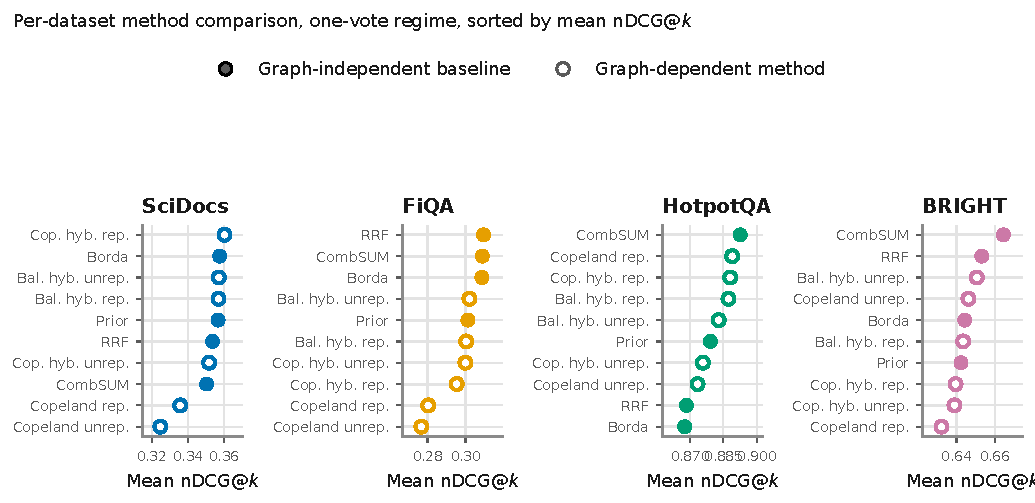
\includegraphics[width=\linewidth]{figures_v2/fig10_baseline_comparison.pdf}
  \caption{Mean nDCG@$k$ under \texttt{ms1}, one panel per dataset, methods
    on the $y$-axis sorted by value; filled markers are the four
    graph-independent baselines (Prior, RRF, CombSUM, Borda), open markers are
    graph-dependent methods. Each panel's $x$-axis is scaled to its own score
    range, so only within-panel comparisons are meaningful. A
    graph-independent baseline is within the top three methods on every
    dataset (CombSUM leads on HotpotQA and BRIGHT, RRF on FiQA), while on
    SciDocs a repaired Copeland-hybrid edges out CombSUM narrowly -- consistent
    with the main paper's macro-average ranking table, which pools
    across all four datasets.}
  \Description{Four horizontal dot plots, one per dataset, each showing ten
    methods' mean nDCG at k under the ms1 regime on the y-axis, sorted from
    lowest to highest. The four graph-independent baselines (CombSUM, RRF,
    Prior, Borda) are drawn as filled markers and appear near the top of the
    ranking in every panel; graph-dependent repaired and unrepaired methods
    are drawn as open markers. A repaired Copeland-hybrid method narrowly
    leads the SciDocs panel; CombSUM or RRF lead the other three panels.}
  \label{fig:supp-mean-ndcg-hybrids}
\end{figure}

Referenced from the main text's ``Raw Versus Normalized Sign Instability''
subsection, which reports the five exact sign-flip values in its own table
and states the aggregate finding (30\% of dataset$\times$regime$\times$pair
cells lack a consistent sign across the three headline protocols, none
individually significant) in prose.

\begin{figure}[h]
  \centering
  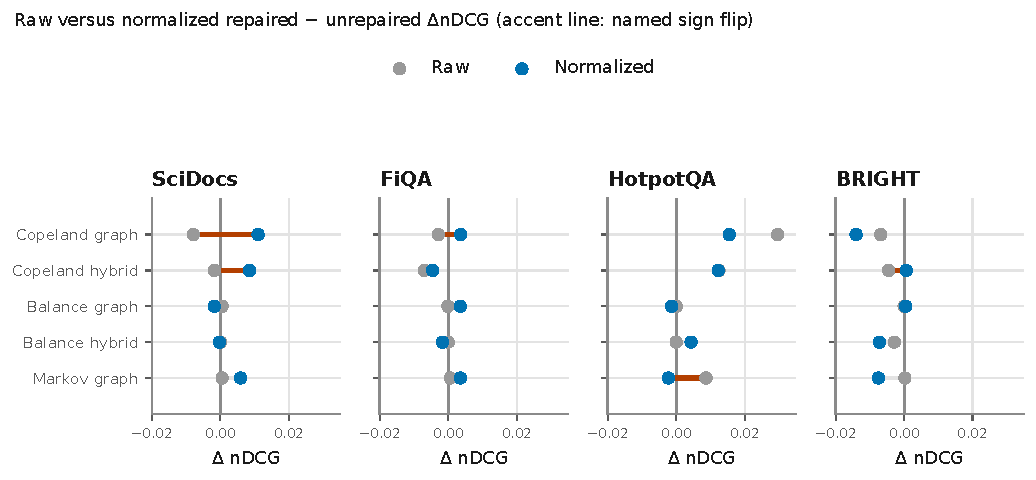
\includegraphics[width=\linewidth]{figures_v2/fig9_sign_change_heatmap.pdf}
  \caption{Repaired-minus-unrepaired $\Delta$nDCG for every method pair under
    \texttt{ms1}, one panel per dataset: gray dot is the raw-margin ablation,
    blue dot is the primary normalized protocol, joined by a line, against a
    zero reference. The five accent-colored lines are the sign flips the main
    paper's raw-vs-normalized sign-flip table reports exactly; other pairs keep
    the same sign or flip only at noise-level magnitude on both sides.}
  \Description{Four panels, one per dataset, each with five rows (one per
    graph-dependent method pair) showing a gray dot for the raw-margin
    ablation and a blue dot for the primary normalized protocol joined by a
    line, plotted against a zero reference line. Five lines across the four
    panels are drawn in a bold accent color to mark the sign flips discussed
    in the text: SciDocs Copeland graph and hybrid, FiQA Copeland graph,
    BRIGHT Copeland hybrid, and HotpotQA Markov graph.}
  \label{fig:supp-raw-calibrated-deltas}
\end{figure}

% =============================================================================
\section{G. LLM Protocol Audit}
\label{sec:supp-llm}

Referenced from the main text's ``Protocol Audit of Stored LLM Judgments''
subsection, which states the headline finding in prose (removing
parser-default and position-bias-driven edges reduces measured cyclicity by
91--100\%, from a 31--62\% cyclic range down to 0--5\%). The table below adds
the two supporting per-corpus statistics not otherwise stated in the main
text: the overall parser default-label rate and the forward/reverse
prompt-order agreement rate. Table~\ref{tab:supp-llm-audit} is the moved
quantitative summary.

\begin{table}[h]
  \caption{Quantitative protocol audit of the stored real-LLM judgment
    corpora (Cohere and Azure OpenAI, FiQA/HotpotQA/BRIGHT, 12{,}020
    responses). Provider-specific detail beyond this summary is in the
    released artifact.}
  \label{tab:supp-llm-audit}
  \begin{tabular}{ll}
    \toprule
    Quantity & Value \\
    \midrule
    Parser default-label rate & 1.1\% overall (0.0\%--3.8\% by provider/dataset) \\
    Position bias, Azure & prefers 1st-shown, 53--58\% \\
    Position bias, Cohere & prefers 2nd-shown, 61--70\% \\
    Forward/reverse agreement & 59--85\% (Cohen's $\kappa$ 0.27--0.71) \\
    Cyclicity after artifact removal & $-$91\% to $-$100\% (31--62\% $\to$ 0--5\%) \\
    \bottomrule
  \end{tabular}
\end{table}

% =============================================================================
\section{H. Full Reproducibility Tables}
\label{sec:supp-reproducibility}

Every canonical aggregate table, protocol manifest, and statistical-family
definition referenced throughout this supplement is released in full in the
accompanying reproducibility artifact (see the main paper's Data Availability
and Reproducibility section); this section does not repeat that inventory.

\bibliographystyle{ACM-Reference-Format}
\bibliography{references}

\end{document}
